\documentclass{beamer}

\usepackage[utf8]{inputenc}

\usepackage{graphicx}
\usepackage{xcolor}
\definecolor{light_red}{RGB}{209,105,81}
\definecolor{light_green}{RGB}{58,181,75}
\definecolor{light_blue}{RGB}{0,153,228}

\setbeamertemplate{frametitle}[default][center]
\setbeamertemplate{navigation symbols}{}
\setbeamerfont{footline}{series=\bfseries}
\setbeamertemplate{footline}[page number]

\usepackage{tikz}
\newcommand{\topline}{%
  \tikz[remember picture, overlay] {%
    \draw[gray, thick] ([xshift = 1cm, yshift = -1.2cm]current page.north west) -- ([xshift = -1cm, yshift = -1.2cm, xshift = \paperwidth]current page.north west);}}

\begin{document}

\begin{frame}
\frametitle{\color{light_red}\textbf{Background}}
\topline

\resizebox{11cm}{!}{
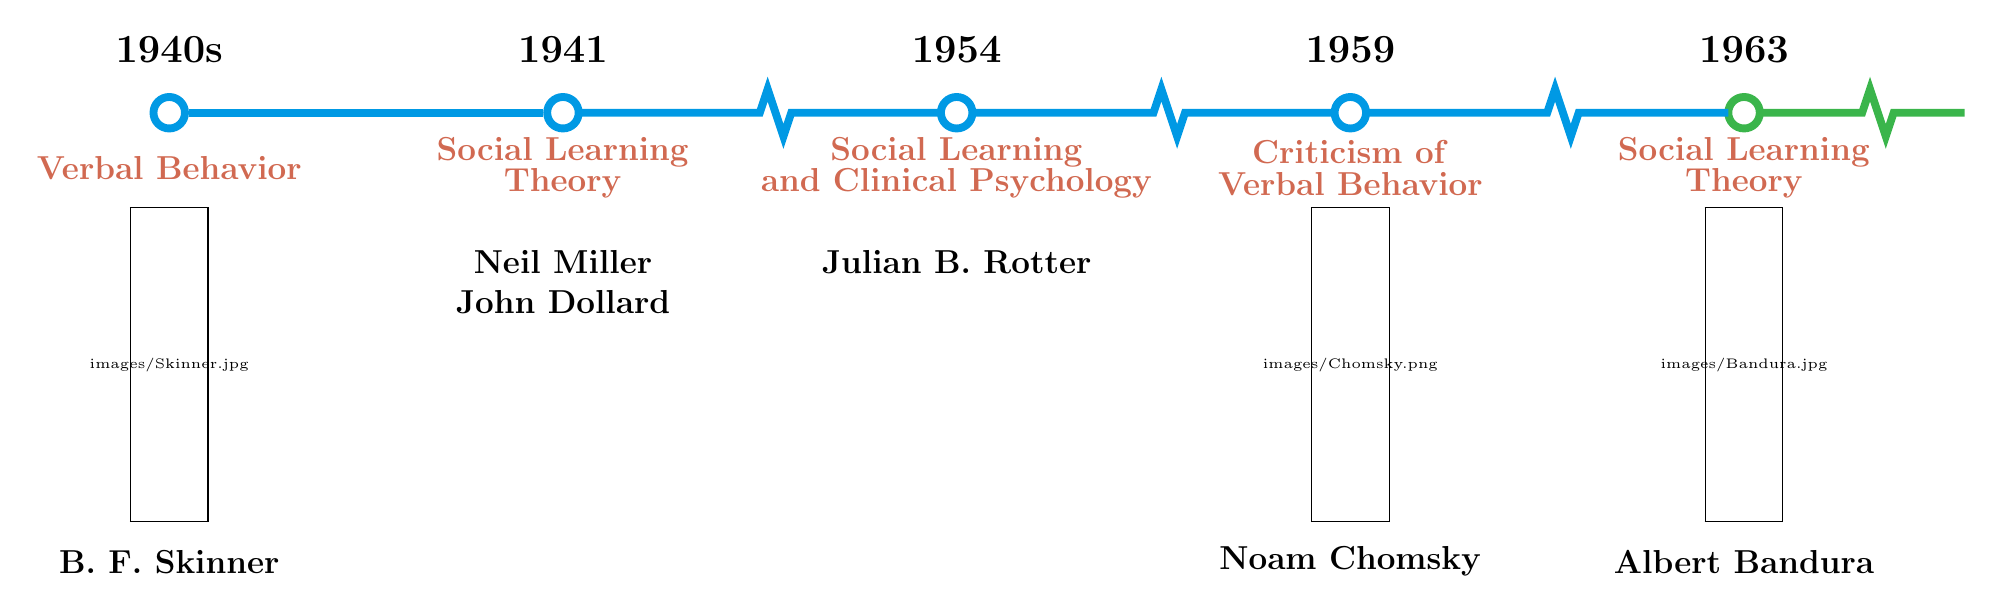
\begin{tikzpicture}

%%% B. F. Skinner %%%
\pgfdeclareimage[height = 4cm]{skinner}{images/Skinner.jpg}
\draw (0, 2.5) node {\color{light_red}\textbf{\large{Verbal Behavior}}};
\node (skinner) at (0, 0) {\pgfuseimage{skinner}};
\draw (0, -2.5) node {\large\textbf{B. F. Skinner}};

\node [circle, line width = 1mm, draw = light_blue, fill = white, minimum size = 0.4cm] (node1) at (0, 3.2) {};
\draw (0, 4) node {\Large\textbf{1940s}};

%%% Social Learning book 1 %%%
\node [circle, line width = 1mm, draw = light_blue, fill = white, minimum size = 0.4cm] (node2) at (5, 3.2) {};
\draw (5, 4) node {\Large\textbf{1941}};
\draw (5, 2.7) node {\color{light_red}\textbf{\large{Social Learning}}};
\draw (5, 2.3) node {\color{light_red}\textbf{\large{Theory}}};
\draw (5, 1.3) node {\large\textbf{Neil Miller}};
\draw (5, 0.8) node {\large\textbf{John Dollard}};

%%% Path between Skinner and Social Learning book 1 %%%
\path [line width = 1mm, draw = light_blue, -] (node1) edge (node2);

%%% Social Learning book 2 %%%
\node [circle, line width = 1mm, draw = light_blue, fill = white, minimum size = 0.4cm] (node3) at (10, 3.2) {};
\draw (10, 4) node {\Large\textbf{1954}};
\draw (10, 2.7) node {\color{light_red}\textbf{\large{Social Learning}}};
\draw (10, 2.3) node {\color{light_red}\textbf{\large{and Clinical Psychology}}};
\draw (10, 1.3) node {\large\textbf{Julian B. Rotter}};

%%% Path between book 1 and book 2 %%%
\draw [line width = 1mm, draw = light_blue]  (5.2, 3.2) -- (7.5, 3.2) -- (7.6, 3.5) -- (7.8, 2.9) -- (7.9, 3.2) -- (9.8, 3.2);

%%% Noam Chomsky %%%
\pgfdeclareimage[height = 4cm]{chomsky}{images/Chomsky.png}
\node (chomsky) at (15, 0) {\pgfuseimage{chomsky}};
\node [circle, line width = 1mm, draw = light_blue, fill = white, minimum size = 0.4cm] (node4) at (15, 3.2) {};
\draw (15, 4) node {\Large\textbf{1959}};
\draw (15, 2.7) node {\color{light_red}\textbf{\large{Criticism of}}};
\draw (15, 2.3) node {\color{light_red}\textbf{\large{Verbal Behavior}}};
\draw (15, -2.5) node {\large\textbf{Noam Chomsky}};

%%% Path between book 2 and Chomsky %%%
\draw [line width = 1mm, draw = light_blue]  (5.2 + 5, 3.2) -- (7.5 + 5, 3.2) -- (7.6 + 5, 3.5) -- (7.8 + 5, 2.9) -- (7.9 + 5, 3.2) -- (9.8 + 5, 3.2);

%%% Albert Bandura %%%
\pgfdeclareimage[height = 4cm]{bandura}{images/Bandura.jpg}
\node (bandura) at (20, 0) {\pgfuseimage{bandura}};
\node [circle, line width = 1mm, draw = light_green, fill = white, minimum size = 0.4cm] (node5) at (20, 3.2) {};
\draw (20, 4) node {\Large\textbf{1963}};
\draw (20, 2.7) node {\color{light_red}\textbf{\large{Social Learning}}};
\draw (20, 2.3) node {\color{light_red}\textbf{\large{Theory}}};
\draw (20, -2.5) node {\large\textbf{Albert Bandura}};

%%% Path between Chomsky and Bandura %%%
\draw [line width = 1mm, draw = light_blue]  (5.2 + 10, 3.2) -- (7.5 + 10, 3.2) -- (7.6 + 10, 3.5) -- (7.8 + 10, 2.9) -- (7.9 + 10, 3.2) -- (9.8 + 10, 3.2);

%%% Path between Chomsky and Bandura %%%
\draw [line width = 1mm, draw = light_green]  (5.2 + 15, 3.2) -- (6.5 + 15, 3.2) -- (6.6 + 15, 3.5) -- (6.8 + 15, 2.9) -- (6.9 + 15, 3.2) -- (7.8 + 15, 3.2);

\end{tikzpicture}
}

\noindent\rule[0ex]{\linewidth}{0.2pt}

\vspace{0.8em}

\small

Contribution of Bandura's Theory:

\vspace{0.5em}

\centering

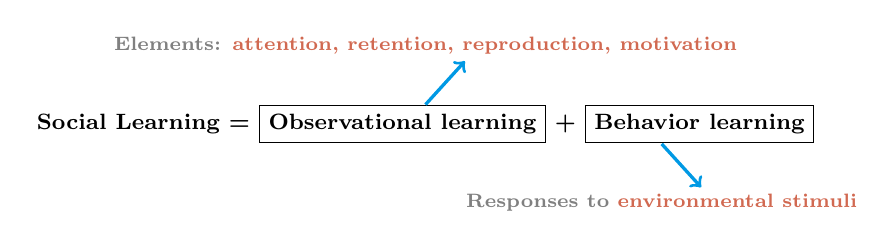
\begin{tikzpicture}
\draw (0, 0) node {\footnotesize\textbf{Social Learning = \fbox{Observational learning} + \fbox{Behavior learning}}};
\draw (0, 1) node {\scriptsize{\textbf{\color{gray}Elements: \color{light_red}attention, retention, reproduction, motivation}}};
\draw [very thick, draw = light_blue, ->]  (0, 0.25) -- (0.5, 0.8);

\draw (3, -1) node {\scriptsize{\textbf{\color{gray}Responses to \color{light_red}environmental stimuli}}};
\draw [very thick, draw = light_blue, ->]  (3, -0.25) -- (3.5, -0.8);

\end{tikzpicture}

\end{frame}


\begin{frame}
\frametitle{\color{light_red}\textbf{Bobo Doll Experiments}}
\topline

\begin{columns}
\begin{column}{0.3\textwidth}
\centering
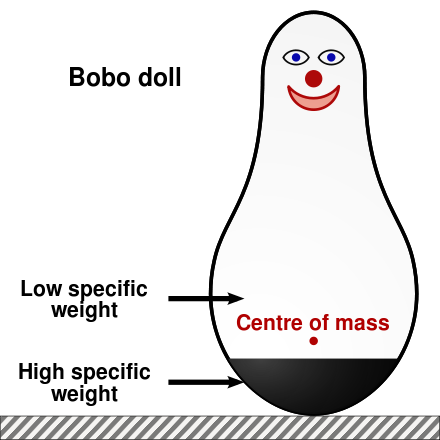
\includegraphics[scale = 0.2]{images/bobo_doll.png}

\end{column}
\begin{column}{0.7\textwidth}
\centering
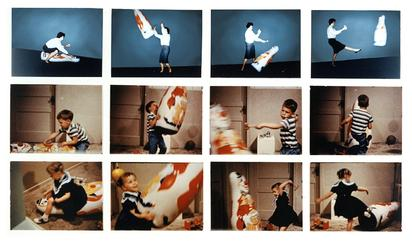
\includegraphics[scale = 0.45]{images/bobo_doll_experiment.jpg}
\end{column}
\end{columns}

\noindent\rule[0ex]{\linewidth}{0.2pt}

\vspace{0.8em}

\small

Contribution of Bandura's Theory:

\vspace{0.5em}

\centering

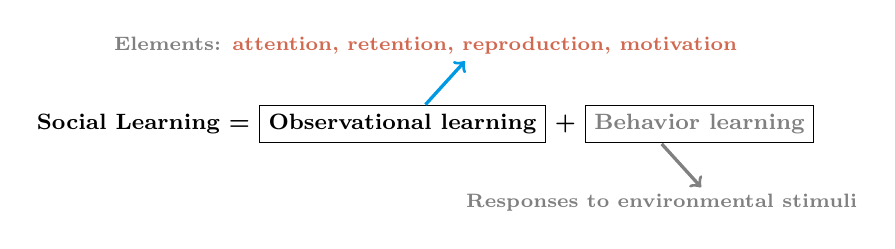
\begin{tikzpicture}
\draw (0, 0) node {\footnotesize\textbf{Social Learning = \fbox{Observational learning} + \fbox{\color{gray}Behavior learning}}};
\draw (0, 1) node {\scriptsize{\textbf{\color{gray}Elements: \color{light_red}attention, retention, reproduction, motivation}}};
\draw [very thick, draw = light_blue, ->]  (0, 0.25) -- (0.5, 0.8);

\draw (3, -1) node {\scriptsize{\textbf{\color{gray}Responses to environmental stimuli}}};
\draw [very thick, draw = gray, ->]  (3, -0.25) -- (3.5, -0.8);

\end{tikzpicture}

\end{frame}

\end{document}